\section{Organización del personal (Gestión del equipo)}
\subsection{Estructura del equipo}
La organización del equipo se basa en una estructura \gls{dd}, la cual ha sido elegida por los integrantes del grupo fundamentándonos en las estructuras de equipo de Mantei.
Para ello nos hemos basado en siete factores para determinar la estructura a elegir: dificultad del problema, tamaño en \gls{ldc} o \gls{pf}, duración del equipo, modularidad del problema, calidad y fiabilidad, fecha de entrega, comunicación requerida en el proyecto.

\begin{figure}[H]
	\centering
	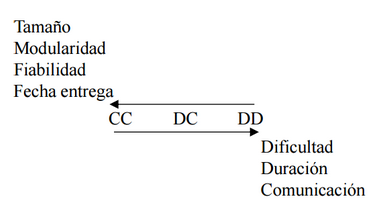
\includegraphics[width=0.6\textwidth]{images/dd.PNG}
	\caption{Tipos de estructura de equipos}
\end{figure}

La estructura de equipo \gls{dd} en la que nos basamos no tiene un líder de grupo permanente, aunque en nuestro caso, \textbf{David Cantador Piedras}, ha realizado el papel de gestor del proyecto, encargado de la organización (distribución del trabajo), motivación y de la resolución de problemas durante el desarrollo del proyecto. Por esa razón, se nombran coordinadores de tareas a corto plazo y se sustituyen por otros para diferentes tareas.

Las decisiones sobre problemas y los enfoques que va a tomar el proyecto, se hacen a consenso del grupo. La comunicación entre los miembros del equipo es horizontal (debido a la ausencia de un líder permanente), gracias a la cual la resolución de dudas o problemas se ve limitada a: compartir información y al apoyo entre los integrantes del grupo.

Por otro lado, conviene resaltar la importancia de la cohesión del grupo, la cual es imprescindible. Un equipo está ``cohesionado'' cuando todos sus miembros comparten un objetivo como enfoque común y luchan por conseguir los resultados deseados para el grupo por encima de los intereses individuales. Además, el respeto, la confianza y la tolerancia son básicas para alcanzar dicha cohesión necesaria, aceptando otros puntos de vista que nos permite enriquecernos y a facilitarnos la resolución de problemas que surjan. Por esa razón, para cada uno de los integrantes se requiere compromiso y esfuerzo, así como la existencia de un proyecto común.

\subsection{Informes de gestión}
Los proyectos de Software se componen de participantes que pueden clasificarse en una de las siguientes cinco categorías:

\begin{itemize}
	\item\textbf{Gestor superior y Gestor técnico del proyecto:}
	      \begin{itemize}
		      \item\textbf{David Cantador Piedras: }es el encargado de definir los aspectos del negocio que a menudo tienen una influencia significativa en el proyecto. Así como, la capacidad de resolver problemas, motivación, planificación y organización del proyecto. Entre sus competencias destacan: Experiencia en desarrollo de aplicaciones Java y C++ (Visual studio code), gestión de MySQL, uso de GIT (software de control de versiones) y conocimientos de IBM RSA (Rational Software Architect) y de Microsoft Proyect.
	      \end{itemize}
	\item\textbf{Profesionales:}
	      \begin{itemize}
		      \item\textbf{Alejandro Barrachina Argudo:} experiencia en desarrollo de aplicaciones Java y C++ (Visual studio code), gestión de MySQL, uso de GIT (software de control de versiones) y conocimientos de IBM RSA (Rational Software Architect) y de Microsoft Proyect.\\
		            Centrado en realizar un breve resumen a modo de introducción del proyecto (objetivos, propósitos…).
		      \item\textbf{Rodrigo Sosa Saéz:} experiencia en desarrollo de aplicaciones Java (Eclipse IDE for Java Developers) y C++, gestión de Oracle SQL Developer, Conocimientos de IBM RSA (Rational Software Architect), uso de GIT (software de control de versiones) y GitHub. \\
		            Centrado en la declaración de los recursos y personal necesarios para el desarrollo del proyecto.
		      \item\textbf{Juan Pantaleón Femenía Quevedo:} experiencia en desarrollo de aplicaciones Java (Eclipse IDE for Java Developers) y C++, uso de GIT (software de control de versiones) y GitHub, gestión de Oracle SQL Developer, Conocimientos de IBM RSA (Rational Software Architect) y Microsoft Proyect.\\
		            Su tarea se centra principalmente en la planificación temporal del trabajo.
		      \item\textbf{David Llanes Martín:} experiencia en desarrollo de aplicaciones Java (Eclipse IDE for Java Developers) y C++, gestión de Oracle SQL Developer, conocimientos de IBM RSA (Rational Software Architect), uso de GIT (software de control de versiones) y GitHub. \\
		            Su tarea está enfocada en la gestión de cambios y seguimiento en el proyecto.
		      \item\textbf{Sergio Sánchez Chamizo:} experiencia en desarrollo de aplicaciones Java (Eclipse IDE for Java Developers) y C++, gestión de Oracle SQL Developer, Conocimientos de IBM RSA (Rational Software Architect), uso de GIT (software de control de versiones) y GitHub y conocimientos de Microsoft Project.\\
		            Su labor está enfocada en la gestión de riesgos del proyecto.
		      \item\textbf{Samuel Rodrigo Moreno:} experiencia en desarrollo de aplicaciones Java (Eclipse IDE for Java Developers) y C++, conocimientos de Microsoft Project, gestión de Oracle SQL Developer, Conocimientos de IBM RSA (Rational Software Architect), uso de GIT (software de control de versiones) y GitHub.\\
		            Centrado en la estimación del proyecto con respecto a su coste, esfuerzo, etc.
		      \item\textbf{Rodrigo Souto Santos:} experiencia en desarrollo de aplicaciones Java (Eclipse IDE for Java Developers) y C++, conocimientos de Microsoft Project, uso de GIT (software de control de versiones), github, gestión de Oracle SQL Developer y conocimientos de IBM RSA (Rational Software Architect). \\
		            Su tarea está centrada en la gestión de los miembros que conforman el equipo de trabajo.
	      \end{itemize}
\end{itemize}

No obstante, todos los integrantes del grupo deberán colaborar en las diferentes partes del proyecto, con el objetivo de obtener un mejor resultado del mismo, además de la tarea explicita para cada uno de los miembros del equipo.

\begin{itemize}
	\item\textbf{Los clientes,} los cuales especifican los requisitos de la aplicación. Mantienen contacto con los profesionales al poderse modificar, añadir algún otro requisito al proyecto.
	\item\textbf{Los usuarios finales, }estarán formados por los trabajadores de las diferentes sucursales de la empresa y los clientes que empleen la aplicación de forma online o que acudan a los establecimientos, los cuales interactuarán con el software.
\end{itemize}
